\documentclass{beamer}

\usepackage{fontspec}
\usepackage{xeCJK}
\setCJKmainfont[BoldFont=Noto Serif CJK TC Bold]{Noto Serif CJK TC}
\XeTeXlinebreaklocale "zh"
\XeTeXlinebreakskip = 0pt plus 1pt
\linespread{1.3}
\allowdisplaybreaks

\usepackage{color}
\usepackage{booktabs}
\usepackage{tabularx}
\usepackage{caption}
\usepackage{tikz}
\usepackage{verbatim}
\usepackage{pgfplotstable}
\pgfplotsset{width=12cm}
\pgfplotsset{height=7cm}
\pgfplotsset{compat=1.13}

\usetheme{EastLansing}
\usetikzlibrary{positioning}
\useinnertheme{rectangles}
\usefonttheme{professionalfonts}

\newcommand{\lw}{0.8mm}
\setbeamercovered{transparent}


%\AtBeginSection[]
%{
  %\begin{frame}<beamer>
	%\frametitle{報告大綱}
	%%\frametitle{RoadMap}
    %\tableofcontents[currentsection]
  %\end{frame}
%}

\title{Paper Report}
\subtitle{\textcolor[rgb]{0.00,0.50,1.00}{{Speech Processing \& Machine Learning Laboratory}}}
\author{徐瑞陽}
\date{2019/09/25}
\begin{document}

\begin{frame}
\maketitle
\end{frame}



\begin{frame}
\frametitle{Outline}
\tableofcontents
\end{frame}

\section{Meta-Learning With Latent Embedding Optimization}
\begin{frame}
  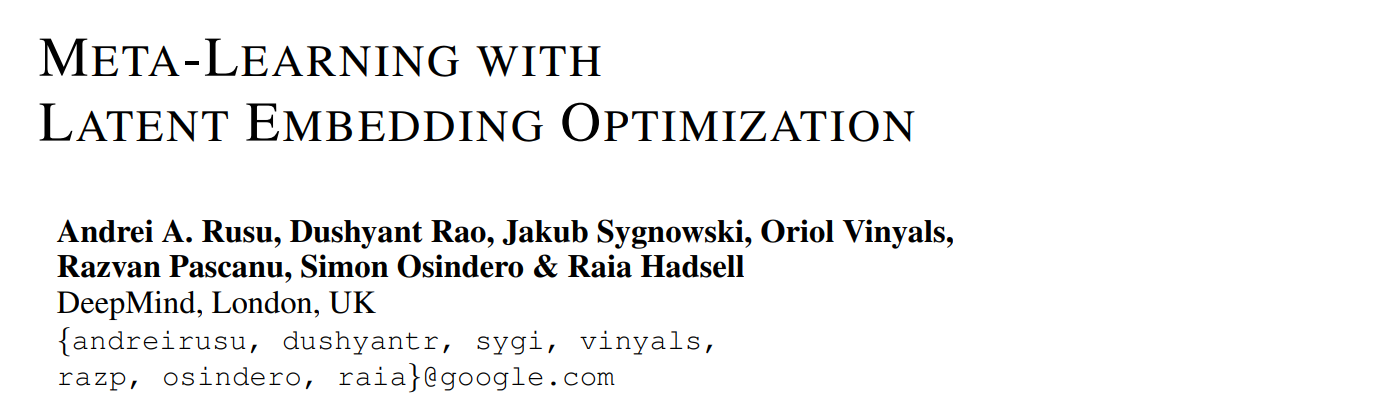
\includegraphics[width=\textwidth]{fig/LEO.png}
  \center ICLR 2019
\end{frame}

\begin{frame}{Motivation}
  Conduct adaptation (inner loop) on high-dimensional parameter space $\Theta$ in low-resource/few-shot regime is hard

  \center Can we conduct on low-dimensional parameter space $\mathcal{Z}$ ? \\ 
  ($\text{dim}(\mathcal{Z}) < \text{dim}(\Theta)$)
\end{frame}

\begin{frame}{Idea}
  \center 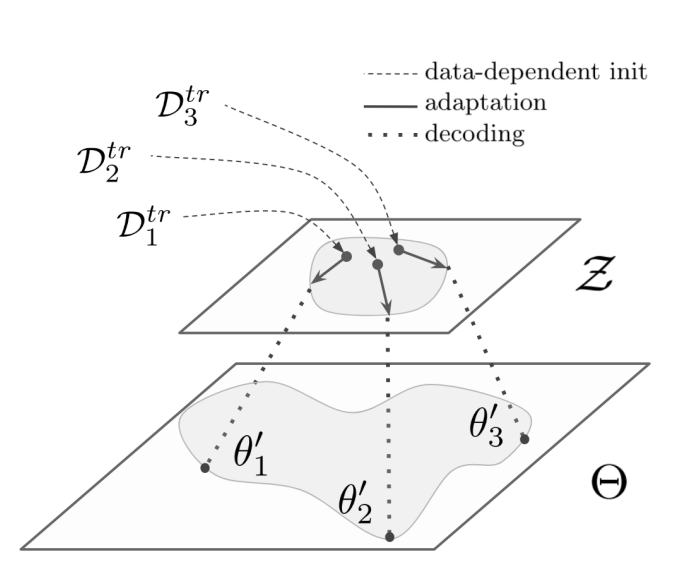
\includegraphics[width=0.7\textwidth]{fig/LEO-idea.png}
\end{frame}

\begin{frame}{Notice}
  \begin{itemize}
    \item \textbf{[Offline]} Pretrain all but last layer using all data (cross tasks in \texttt{meta-train})
    \item \textbf{[Meta-learn]} Output softmax layer
    \item \textbf{[Task Conditioning]} Latent embedding $z$ conditions on task $T$
  \end{itemize}
\end{frame}

\begin{frame}{Structure}
  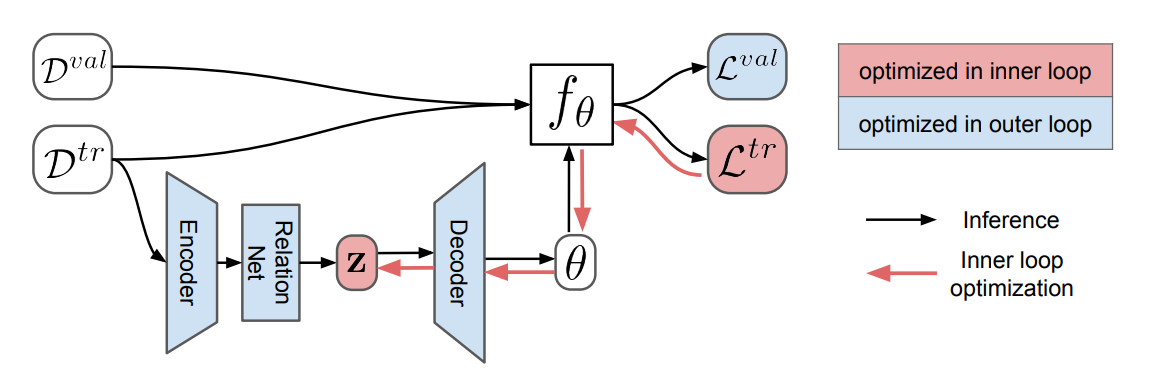
\includegraphics[width=\textwidth]{fig/LEO-struct.png}
\end{frame}

\begin{frame}{Implementation}
  Given task $T = (\mathcal{D}^{tr}, \mathcal{D}^{val})$, which is $N$-way, $K$-shot, we want to learn $f(\theta)$ as follows
  \[
    W = \begin{bmatrix}
    \textemdash \quad w_1 \quad \textemdash  \\
    \textemdash \quad w_2 \quad \textemdash \\
    \cdot\\
    \cdot\\
    \cdot\\
    %\hdotsfor{5} \\
    \textemdash \quad w_N \quad \textemdash\\
\end{bmatrix}
\]
\center in latent space $\mathcal{Z}$
\end{frame}

\begin{frame}{Bridge between $w_n$ and $z_n$}
Parameter
\begin{itemize}
  \item Encoder: $g_{\phi_e}$: $\mathcal{X} \rightarrow \mathcal{H}$
  \item Relation Network $g_{\phi_r}$: $\mathcal{H} \times \mathcal{H} \rightarrow \mathcal{Z}$
  \item Decoder (parameter generator) $g_{\phi_d}$: $\mathcal{Z} \rightarrow \Theta$
\end{itemize}
\end{frame}

\begin{frame}{Bridge between $w_n$ and $z_n$}
  Encoding
  \begin{center}
    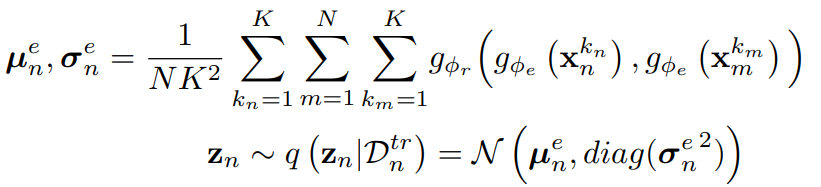
\includegraphics[width=0.8\textwidth]{fig/LEO-encoding.png}
  \end{center}

  Decoding
  \begin{center}
  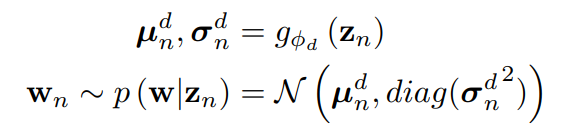
\includegraphics[width=0.6\textwidth]{fig/LEO-decoding.png}
  \end{center}
\end{frame}

\begin{frame}{Inner Loop Optimization through LEO}
  Objective
  \begin{center}
  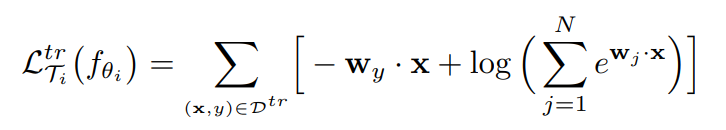
\includegraphics[width=0.6\textwidth]{fig/LEO-inner-obj.png}
  \end{center}

  \begin{itemize}
    \item Compute loss w.r.t $\theta$
    \item Perform gradient step w.r.t $z$ \\
      $z^\prime \leftarrow z - \alpha \nabla_z \mathcal{L}^{tr}_{T}(f_{\theta})$

  \end{itemize}
\end{frame}

\begin{frame}{Outer Loop Optimization}
  %meta-param $\phi = \lbrace \phi_e, \phi_r, \phi_r \rbrace$
  Objective

  \center 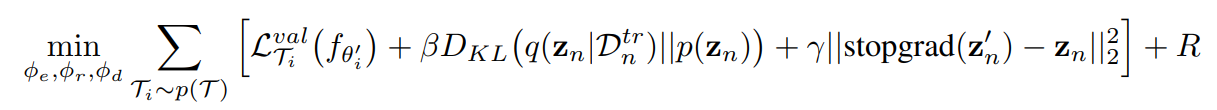
\includegraphics[width=1.0\textwidth]{fig/LEO-outer-obj.png}
  %meta-learn parameter $\phi = \lbrace \phi_e, \phi_r, \phi_d \rbrace$
  \begin{itemize}
    \item $p(z_n) = \mathcal{N}(0,\mathcal{I})$
    \item Encourage encoded initialization $z$ is close to adapted embedding $z^\prime$ \\
      (to minimize traverse length)
    \item $L_2$ regularization of $\phi$
  \end{itemize}
\end{frame}

\begin{frame}{Result on miniImageNet}
  \center 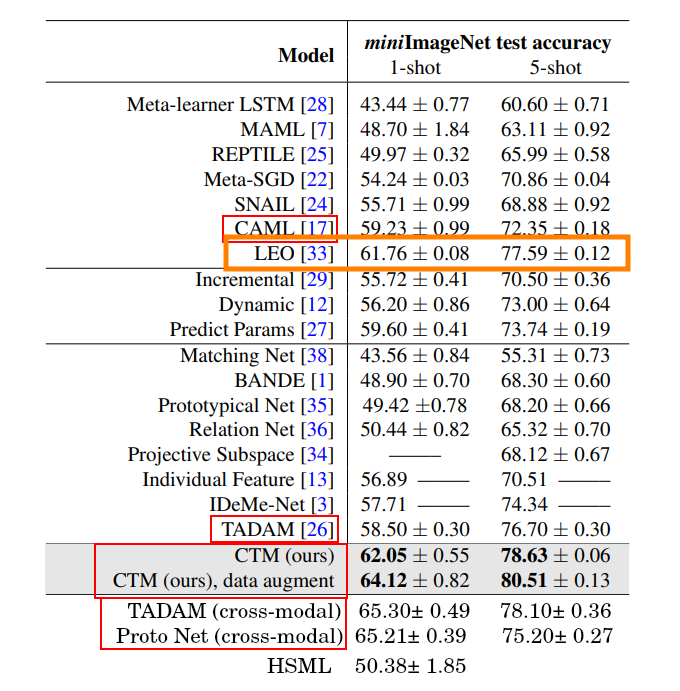
\includegraphics[width=0.7\textwidth]{fig/LEO-result.png}
\end{frame}

%\section{MISC}
\begin{frame}
	\begin{center}
    %\weib{\LARGE{謝謝聆聽!}}
    \LARGE{Questions?}
	\end{center}
\end{frame}

\end{document} 
